\documentclass[12pt]{article}
\usepackage{geometry}
\geometry{a4paper, total={170mm,257mm},left=20mm, top=10mm,}
\usepackage[colorlinks=true,linkcolor=blue,urlcolor=black]{hyperref}
\usepackage{bookmark}
\usepackage{pdfpages}
\begin{document}
\title {Labtainer Student Guide}
\maketitle

\section {Introduction}
This manual is intended for use by students performing labs with Labtainers.
Labtainers assume you have a Linux system, e.g., a virtual machine.  Refer to
in Appendix A for installation of Virtual Box and a Linux system.
Note that any Linux system can be used as long as it supports Dockers.

\subsection{Obtaining Labtainers and installing Docker}
The Labtainers environment is distributed as a tarball from:
\url{https://my.nps.edu/web/cisr/labtainers}
Untar this file in your Linux system.

Install Docker by running one of the install-docker scripts, depending on your Linux
distribution:
\begin{verbatim}
    ./labtainer/trunk/setup_scripts/install-docker-ubuntu.sh
    ./labtainer/trunk/setup_scripts/install-docker-fedora.sh
    ./labtainer/trunk/setup_scripts/install-docker-debian.sh
    ./labtainer/trunk/setup_scripts/install-docker-centos.sh
\end{verbatim}
If you have a different Linux distribution, find instructions for installing Docker-ce at
\url{https://docs.docker.com/engine/installation/}

If you already have Docker installed, or installed Docker for a different distribution,
make sure you also have python, and
the python \textit{netaddr} module installed.  Be sure you have at least version 17.06.0-ce of Docker.
If you have Docker installed on Ubuntu, you
may need to run:
\begin{verbatim}
    ./labtainer/trunk/setup_scripts/fixresolv.sh
\end{verbatim}
\noindent Also note that older Linux distributions, e.g., Ubuntu 14.* lack the
\textit{realpath} package, which should be installed prior to using Labtainers.

\section{Performing a Lab}
All labs are run from the same Labtainer workspace directory:
\begin{verbatim}
    cd labtainer/trunk/scripts/labtainer-student
\end{verbatim}
\noindent Then run the lab:
\begin{verbatim}
    ./start.py <labname>
       where <labname> is the name of the lab to run.  Leaving this out will 
       display a list of available labs.
\end{verbatim}

The first time any given lab is run, it may take a short while to build the Docker images 
required for the lab.  Subsequent runs will start much faster.

Follow the instructions that appear in one of the resulting virtual terminals.  Please
note that some of the initial lab instructions repeat the steps you've already taken, and you need
not repeat those.  While running the lab, if you require more virtual terminals, use:
\begin{verbatim}
    ./moreterm.py <labname> <container>
    where <container> is the host name of the component on which to attach a terminal.  
    It can be omitted for labs having a single component.
\end{verbatim}

The virtual terminals for most labs present bash shells via which you can interact
with the attached computer, (which is actually a Docker container designed to appear
like a separate computer).  A single computer
may have multiple virtual terminals attached to it.  Each computer is independent, and 
may use networks to interact with other computers within the lab.  

\subsection{Networking}
In addition to network properties defined for the lab,
each component \texttt{/etc/host} file includes a "my\_host entry" that names
the host Linux.  Most containers will include a default gateway that
leads to the Linux host.  This allows students to scp files to/from the container and host.
It also allows the student to reach external networks, e.g., to fetch additional packages in
support of student exploration.

In some instances, the lab requires one or more components to a have different default route.
Typically, these components will include a \textit{togglegw.sh} script that the student
can use to toggle the default gateway between one that leads to the host, and one defined for the lab.
This allows students to add packages on components having lab-specific default gateways.
Use of the \textit{togglegw.sh} script is not necessary to reach the Linux host, (e.g., to scp files).

\subsection{Limitations}
The Labtainer "computers" are individual Docker containers that are interconnected via virtual
networks.  These containers each share the Linux kernel of your host.  Thus, a change
to the kernel configuration on one computer, (e.g., enabling ASLR), will be visible on
other containers, as well as your host.

The computers each include a ".local" directory beneath the HOME directory.  This is used
by the Labtainer framework and includes results that get packaged up for forwarding to the
instructor.  Do not modify any files beneath the .local directory.  Otherwise, you can treat
those containers as Linux systems, and explore them.

Please note that while running some programs in the Labtainer computers, passwords provided to
applications such as "ssh" are not supressed.  This is a side effect of the Labtainer
support for automated assessment.  

\subsection{Stopping Labtainers}
When you are finished, or wish to stop working, type:
\begin{verbatim}
    ./stop.py <labname>
\end{verbatim}
The stop.py command will display the directory containing a zip file that should be provided to your instructor.

\appendix 
\section {Appendix A: Installing Virtual Box and Ubuntu}
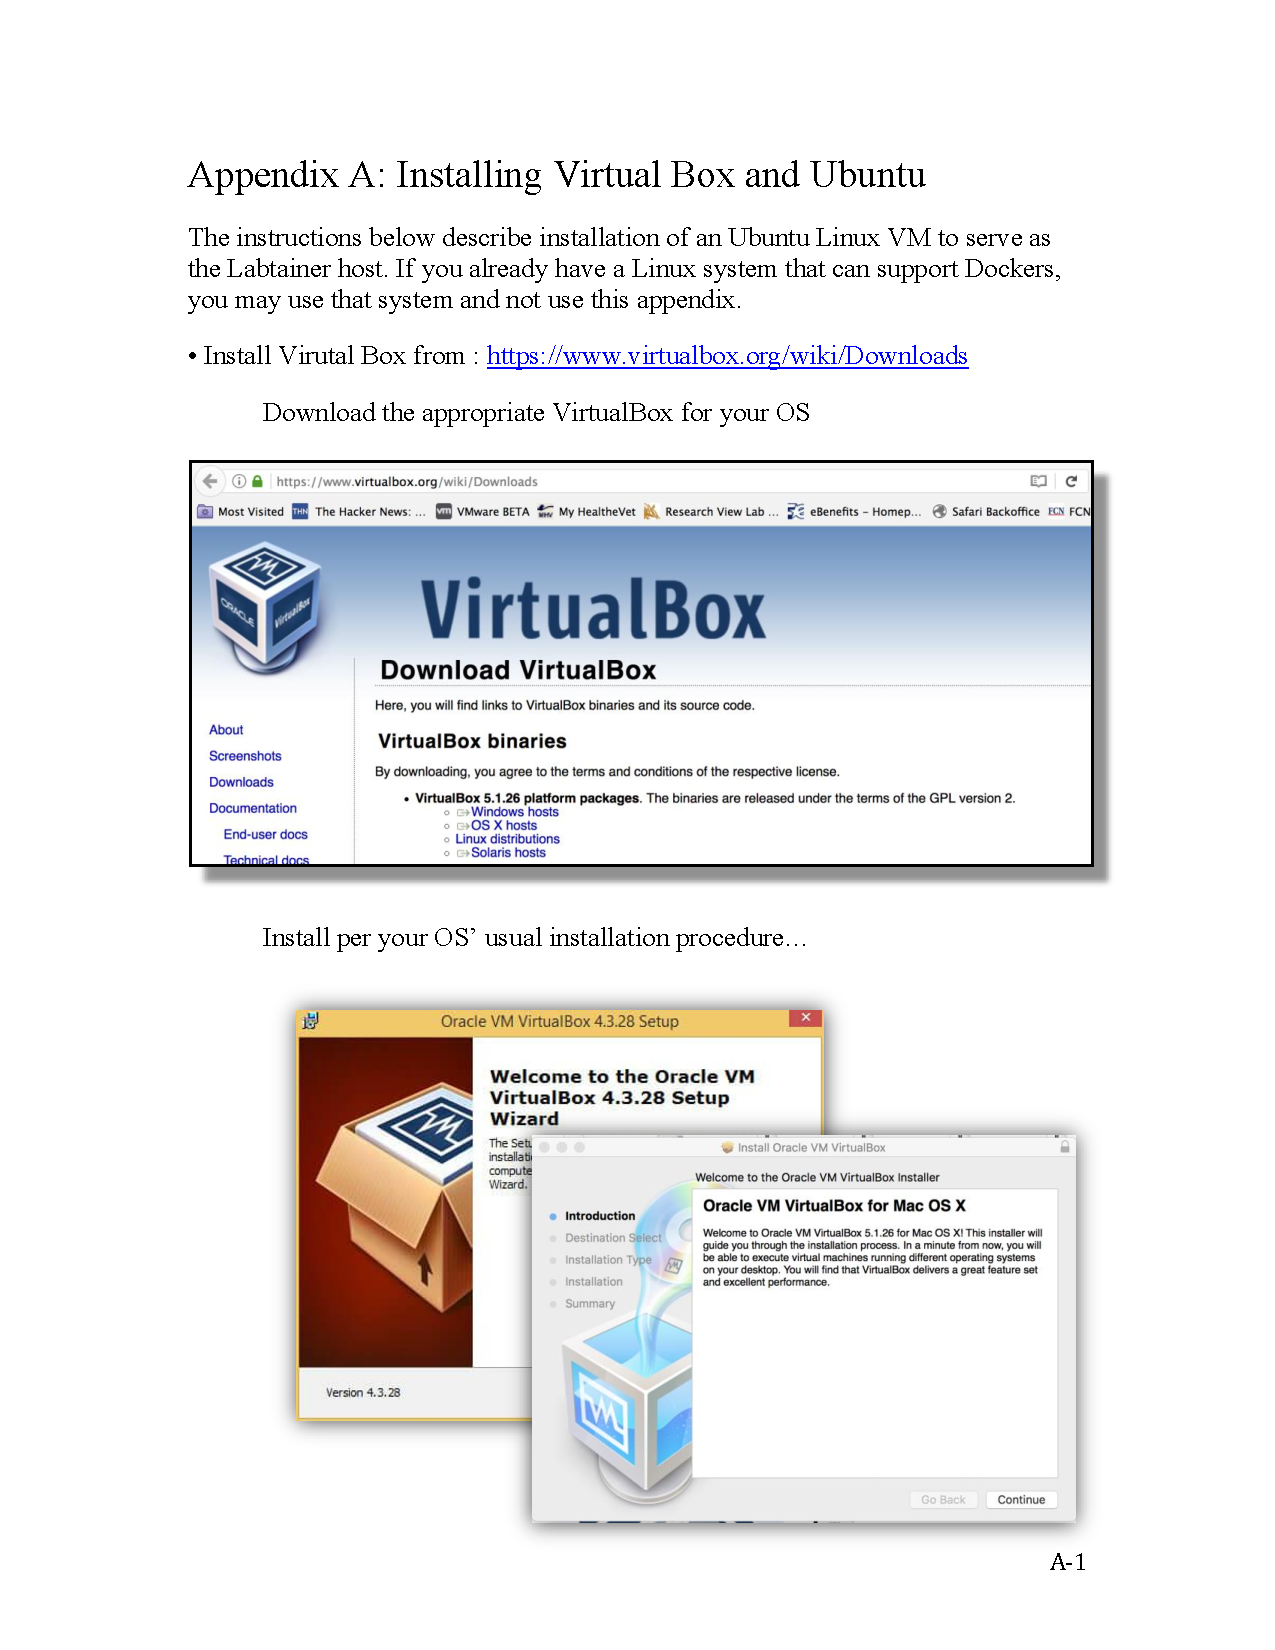
\includepdf[pages=-]{InstallingVB-Linux.pdf}
\appendix 
\section {Appendix B: Labtainer Command Summary}
\label{sec:appendixB}
The following labtainer commands are available from the \texttt{labtainer/trunk/scripts/labtainer-student}
directory:
\begin{itemize}
\item \texttt{./start.py <lab> --}
Start the named lab.  If no name is given, a list of available labs will be displayed.
\item \texttt{./stop.py <lab> --} Stop the named lab.
\item \texttt{./moreterm.py <lab> <container> --} create a new virtual terminal for the container.
\item \texttt{./redo.py <lab> --}
Delete any previous containers associated with this lab and start it fresh.  \textbf{Warning}: this will lose any
previous data from the named lab.
\end{itemize}

Most labs display lab instructions in one of the windows that appears after the lab starts.  If those instructions
stop displaying, e.g., because "q" is pressed in that window, then type the following in that window:
\begin{verbatim}
    less instructions.txt
\end{verbatim}


\end{document}
